%%%%%%%%%%%%%%%%%%%%%%%%%%%%%%%%%%%%%%%%%
% a0poster Portrait Poster
% LaTeX Template
% Version 1.0 (22/06/13)
%
% The a0poster class was created by:
% Gerlinde Kettl and Matthias Weiser (tex@kettl.de)
% 
% This template has been downloaded from:
% http://www.LaTeXTemplates.com
%
% License:
% CC BY-NC-SA 3.0 (http://creativecommons.org/licenses/by-nc-sa/3.0/)
%
%%%%%%%%%%%%%%%%%%%%%%%%%%%%%%%%%%%%%%%%%

%----------------------------------------------------------------------------------------
%	PACKAGES AND OTHER DOCUMENT CONFIGURATIONS
%----------------------------------------------------------------------------------------

\documentclass[a0,portrait]{a0poster}

\usepackage{multicol} % This is so we can have multiple columns of text side-by-side
\columnsep=100pt % This is the amount of white space between the columns in the poster
\columnseprule=3pt % This is the thickness of the black line between the columns in the poster

\usepackage{algorithm,algpseudocode,ifpdf}


\usepackage[svgnames]{xcolor} % Specify colors by their 'svgnames', for a full list of all colors available see here: http://www.latextemplates.com/svgnames-colors

\usepackage{times} % Use the times font
%\usepackage{palatino} % Uncomment to use the Palatino font

\usepackage{graphicx} % Required for including images
\graphicspath{{figures/}} % Location of the graphics files
\usepackage{booktabs} % Top and bottom rules for table
\usepackage[font=small,labelfont=bf]{caption} % Required for specifying captions to tables and figures
\usepackage{amsfonts, amsmath, amsthm, amssymb} % For math fonts, symbols and environments
\usepackage{wrapfig} % Allows wrapping text around tables and figures

\newcommand{\argmin}[1]{\underset{#1}{\operatorname{argmin}}\text{ }}
\newcommand{\argmax}[1]{\underset{#1}{\operatorname{argmax}}\text{ }}


\begin{document}

%----------------------------------------------------------------------------------------
%	POSTER HEADER 
%----------------------------------------------------------------------------------------

% The header is divided into two boxes:
% The first is 75% wide and houses the title, subtitle, names, university/organization and contact information
% The second is 25% wide and houses a logo for your university/organization or a photo of you
% The widths of these boxes can be easily edited to accommodate your content as you see fit

\begin{minipage}[b]{0.75\linewidth}
\veryHuge \color{NavyBlue} \textbf{Near Field Cosmology with RR Lyrae Variables} \color{Black}\\ % Title
\Huge\textit{Building and Testing Parsimonious Models}\\[2cm] % Subtitle
\huge \textbf{James Long \& Jennifer Marshall \& Lucas Macri}\\[0.5cm] % Author(s)
\huge Texas A\&M University, Department of Statistics and Physics \& Astronomy\\[0.4cm] % University/organization
\Large \texttt{jlong@stat.tamu.edu}\\% --- 1 (000) 111 1111\\
\end{minipage}
%
\begin{minipage}[b]{0.25\linewidth}
\includegraphics[width=20cm]{tamu.png}\\
\end{minipage}

\vspace{1cm} % A bit of extra whitespace between the header and poster content

%----------------------------------------------------------------------------------------

\begin{multicols}{2} % This is how many columns your poster will be broken into, a portrait poster is generally split into 2 columns


%----------------------------------------------------------------------------------------
%	INTRODUCTION
%----------------------------------------------------------------------------------------

\section*{Motivation}

\begin{itemize}
\item Cosmological simulations predict the existence of many dwarf satellite galaxies.
\item Few Milky Way satellite galaxies have been observed: \textbf{Missing satellites problem} \cite{kauffmann1993formation,klypin1999missing,moore1999dark}
\item Finding satellite galaxies is difficult due to low surface brightness and diffuse nature.
\item Distance determination to structures in the Milky Way halo is difficult.
\item Finding RR Lyrae in halo enables distance determination, detection of structure. \cite{baker2015charting}
\end{itemize}



\section*{RR Lyrae in the Dark Energy Survey}

\begin{itemize}
\item Easy to estimate parameters for well observed RR Lyrae. For example with $>50$ observations per filter we used the Generalized Lomb Scargle to determine the period for an RR Lyrae observed by SDSS-III in Stripe 82. Based on the folded light curve, the period estimate appears correct:

\begin{center}\vspace{1cm}
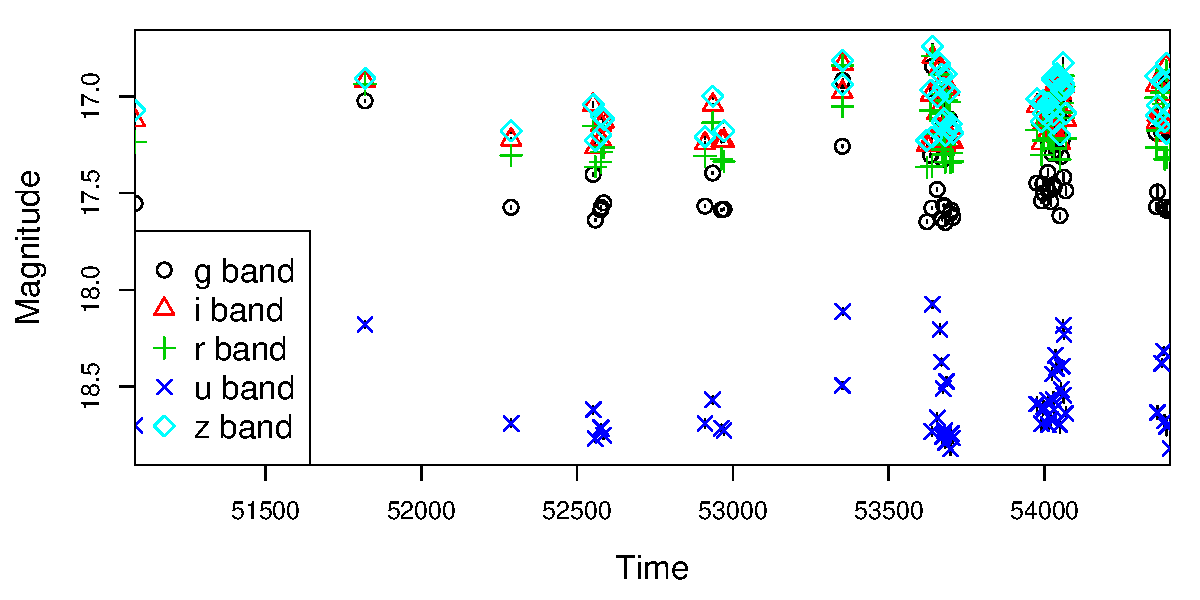
\includegraphics[width=0.49\linewidth]{unfolded.pdf}
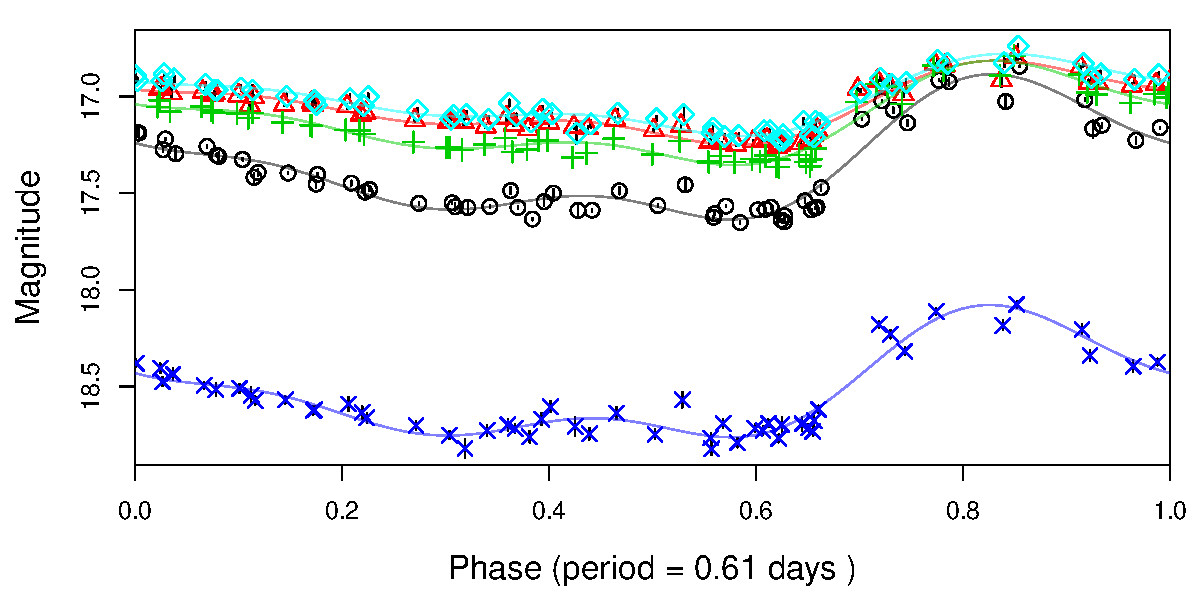
\includegraphics[width=0.49\linewidth]{folded.pdf}
\captionof{figure}{An SDSS Stript 82 RR Lyrae unfolded (left) and folded (right) observed in bands $g,i,r,u,z$. The fitted curves use the Generalized Lomb Scargle (GLS) method for estimating period. This method works well when light curves are well sampled, but poorly for sparsely sampled light curves like those collected by Pan--STARRS and DES.}
\end{center}\vspace{1cm}


\item The \textbf{Dark Energy Survey} (DES) will sparsely sample RR Lyrae. An example of this type of sampling is shown in Figure \ref{fig:panstarrs}.

\begin{center}\vspace{1cm}
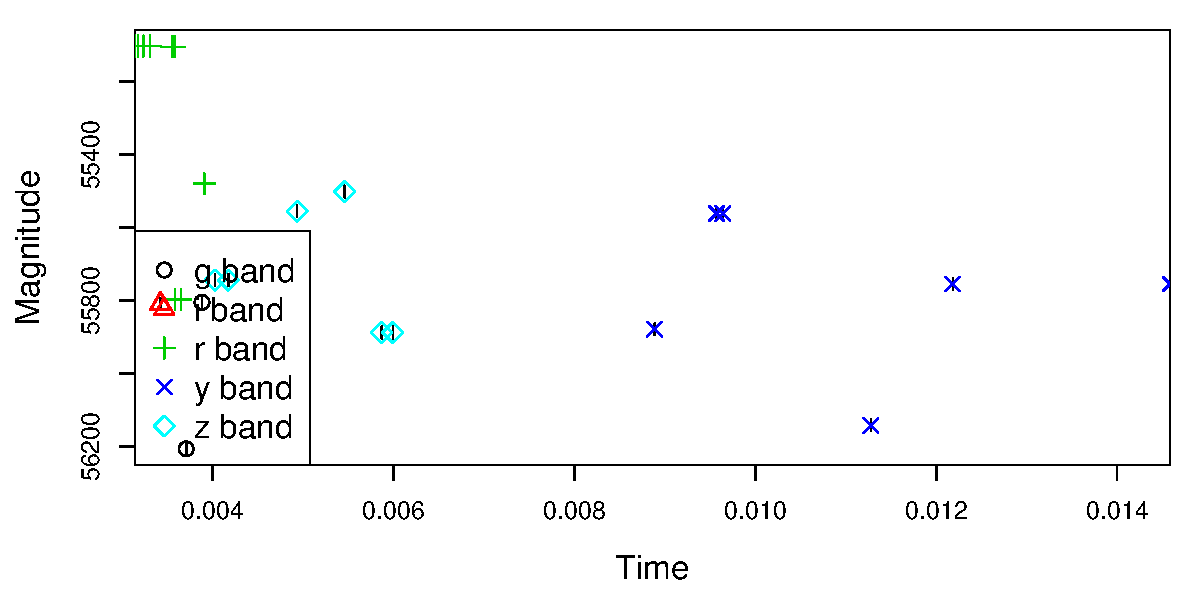
\includegraphics[width=0.5\linewidth]{unfolded_panstarrs.pdf}
\captionof{figure}{A Pan--STARRS RR Lyrae. The Dark Energy Survey (DES) is collecting similar quality light curves. \cite{hernitschek2016finding} \label{fig:panstarrs}}
\end{center}\vspace{1cm}


\item Distance determination using RR Lyrae requires identifying light curves as RR Lyrae and estimating parameters such as period. This is difficult with light curves sampled at the quality of Figure \ref{fig:panstarrs}. Methods such as Generalized Lomb Scargle (GLS), which work well (estimate period correctly with high probability) for well--observed light curves, perform poorly for sparsely observed light curves.


\end{itemize}


\section*{RR Lyrae Model Constructed with SDSS Stripe 82 Data}

\begin{itemize}
\item Proposed model: The brightness in band $b$ at time $t$ is

{\Large
\begin{equation*}
m_b(t) = \alpha + \beta_b + E[B-V]\delta_b + a\gamma_b(\omega t + \phi)
\end{equation*}
}

where the \underline{global parameters} common for all RR Lyrae are
\begin{align*}
\beta_b &=  \text{ magnitude off--set in band $b$ }\\
\delta_b &= \text{ attenuation caused by dust in band $b$ }\\
\gamma_b &= \text{ normalized shape of light curve in band $b$ }\\
\end{align*}
and the \underline{individual parameters} specific to each RR Lyrae are
\begin{align*}
\alpha &= \text{ mean brightness across all bands }\\
E[B-V] &= \text{ amount of dust }\\
a &= \text{ amplitude of variation }\\
\omega &= \text{ frequency of variation }\\
\phi &= \text{ phase of variation }
\end{align*}

This is a \underline{parsimonious} model because it only has five free parameters to fit to each star.

\item For a specific RR Lyrae the data is $\{\{(m_{jb},t_{jb},\sigma_{jb})\}_{j=1}^{n_b}\}_{b=1}^B$ where $B$ is the number of filters and $m_{jb}$ is the star brightness measured at time $t_{jb}$ with uncertainty $\sigma_{jb}$ in band $b$. The data is connected to the model through
\begin{equation*}
m_{jb} = m_b(t_{jb}) + \epsilon_{jb}
\end{equation*}
where $\epsilon_{jb} \sim N(0,\sigma_{jb}^2)$. 

\item \underline{Global parameters} are estimated from a set of 309 well--observed SDSS Stripe 82 RR Lyrae AB \cite{sesar2010light}. For example the $\gamma_b$ (functional) parameters are shown in Figure \ref{fig:gamma}. 

\begin{center}\vspace{1cm}
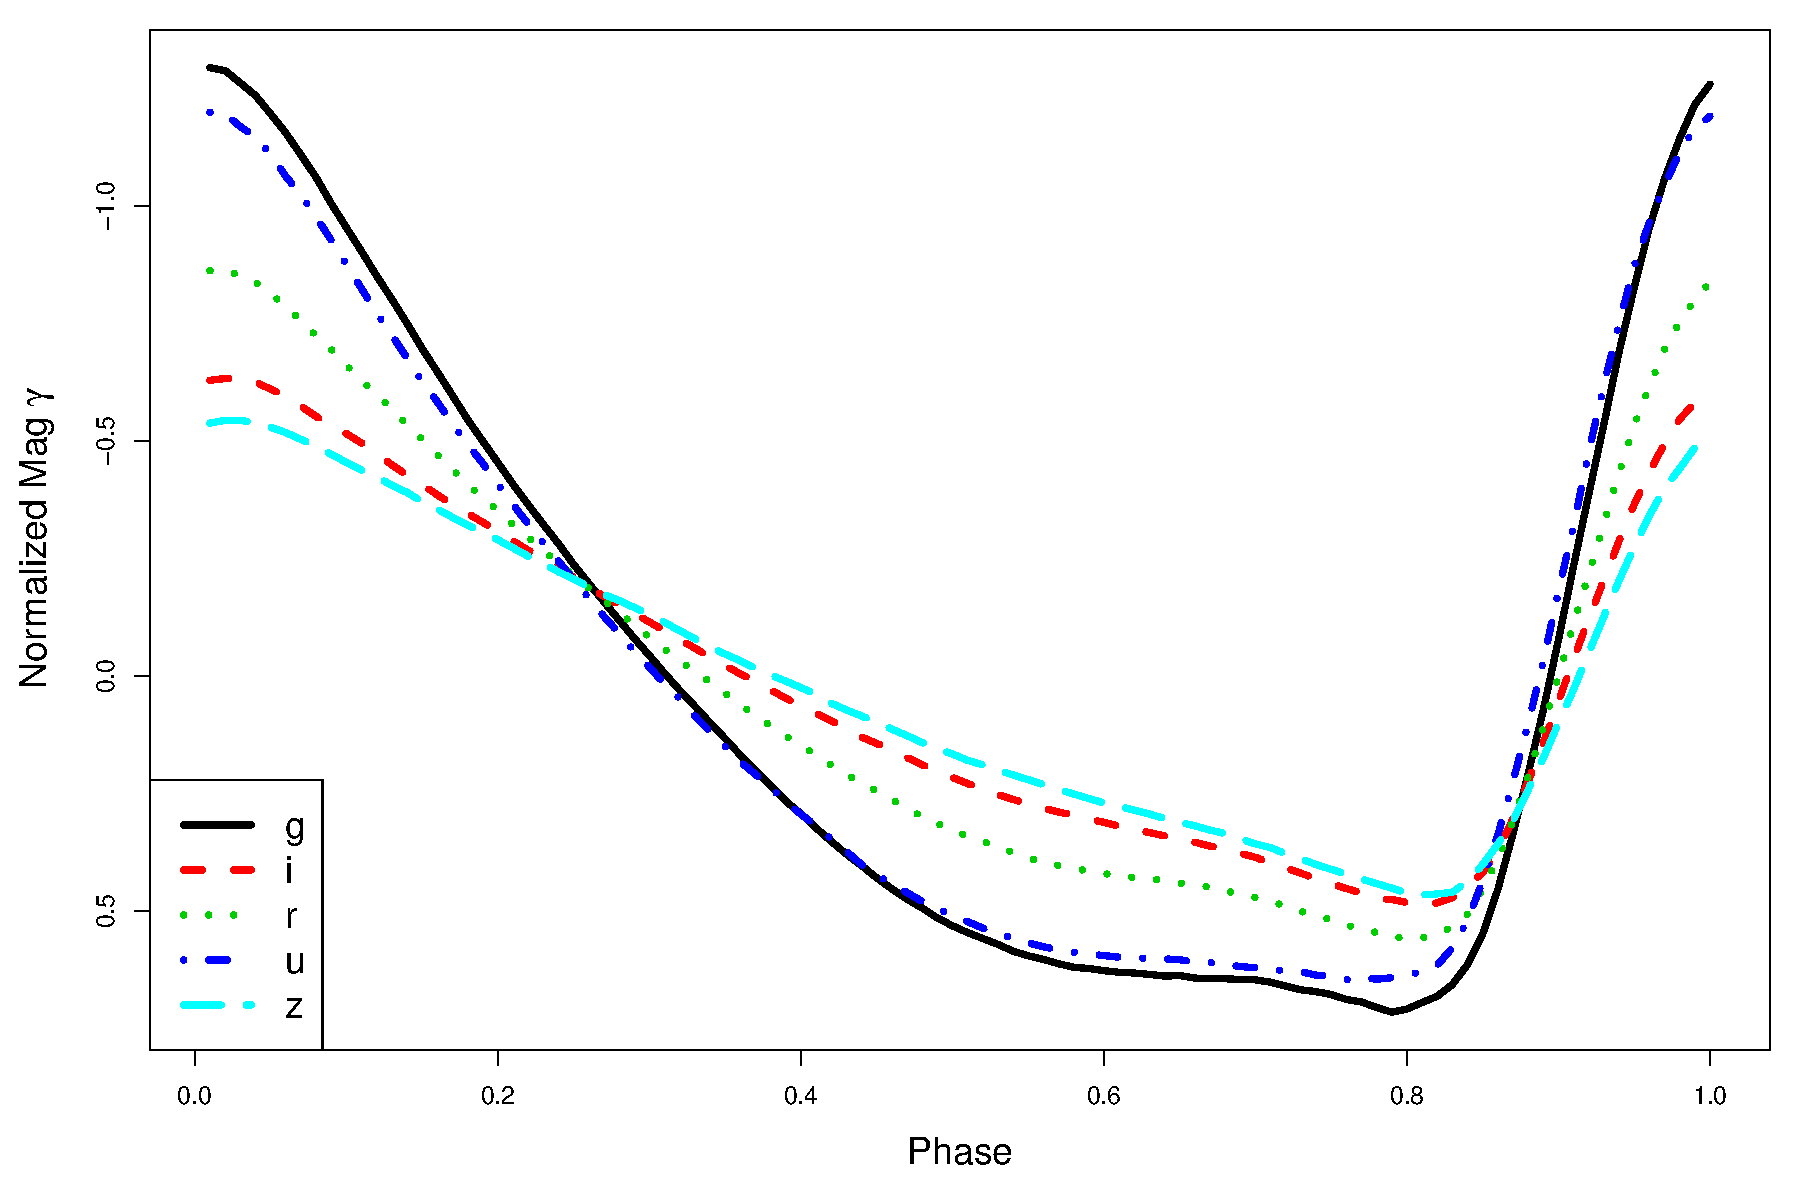
\includegraphics[width=0.55\linewidth]{templates.pdf}
\captionof{figure}{$\gamma_b$ functions for bands $b=g,i,r,u,z$ estimated from SDSS Stripe 82 RR Lyrae. \label{fig:gamma}}
\end{center}\vspace{1cm}


\end{itemize}

%%% results table

\section*{Fitting Model to Light Curve}

\begin{itemize}

\item Define

\begin{equation*}
g(\omega,\alpha,E[B-V],a,\phi) = \sum_{b=1}^B \sum_{j=1}^{n_b}\left(\frac{m_{jb} - \alpha - E[B-V]d_b - a\gamma_b(\omega t_{jb} + \phi)}{\sigma_{bi}}\right)^2
\end{equation*}

\item Estimate parameters through maximum likelihood:
\begin{itemize}
\item Likelihood is highly multimodal in $\omega$, so perform grid search on frequency.
\item Model is linear in $\alpha$,$E[B-V]$, and $a$, so closed form updates.
\item Newton--Raphson updates for $\phi$ parameter.
\end{itemize}

\item Pseudocode

\begin{algorithmic}[1]
  \State $\Omega \gets (\omega_1,\ldots,\omega_N)$ \Comment{Grid for Frequency}
  \State $\phi \gets Unif[0,1]$ \Comment{Random Initial Phase}
  \For{$k = 1,\ldots,N$}
  \For{$l = 1,\ldots,10$}
  \State $\alpha,E[B-V],d \gets \argmin{\alpha,E[B-V],a} g(\omega,\alpha,E[B-V],a,\phi)$  \Comment{Closed form solutions}
  \State $\phi = \phi - \left[\frac{d^2}{d\phi^2}g(\omega_k,\alpha,E[B-V],a,\phi)\right]^{-1}\left[\frac{d}{d\phi}g(\omega_k,\alpha,E[B-V],a,\phi)\right] $ \Comment{Newton update for $\phi$}
  %% \State $p \gets p + 1$
  %% %% \Until{$||\theta_{l,p} - \theta_{l,p-1}|| < \epsilon$}
  %% \State $\theta_{l} \gets \theta_{l,p}$
  \EndFor
  \State $\text{RSS}(\omega_k) = g(\omega_k,\alpha,E[B-V],a,\phi)$
  \EndFor
  \State $\widehat{\omega} = \min \text{RSS}(\omega)$
\end{algorithmic}

\end{itemize}


\section*{Results}

\begin{itemize}

\item We conduct a simulation study to compare model performance to the Generalized Lomb Scargle (GLS) method for estimating periods. GLS models the light curve as a sinusoid function.

\item We downsampled a set of 350 SDSS-III Stripe 82 RR Lyrae to 50 observations (total across all bands) and then computed the fraction of time each method estimated the period correctly (within $0.2\%$) or the true period was within the top five candidate periods given by the method.

\begin{center}
\begin{tabular}{l l l}
\toprule
\textbf{Method} & \textbf{Correct} & \textbf{Correct in Top 5}\\
\midrule
RR Lyrae Model  & 0.89 & 0.99 \\
Generalized Lomb Scargle & 0.49  &  0.90\\
\bottomrule
\end{tabular}
\end{center}

\item Example of model fit to downsampled SDSS Stripe 82 RR Lyrae.

\begin{center}\vspace{1cm}
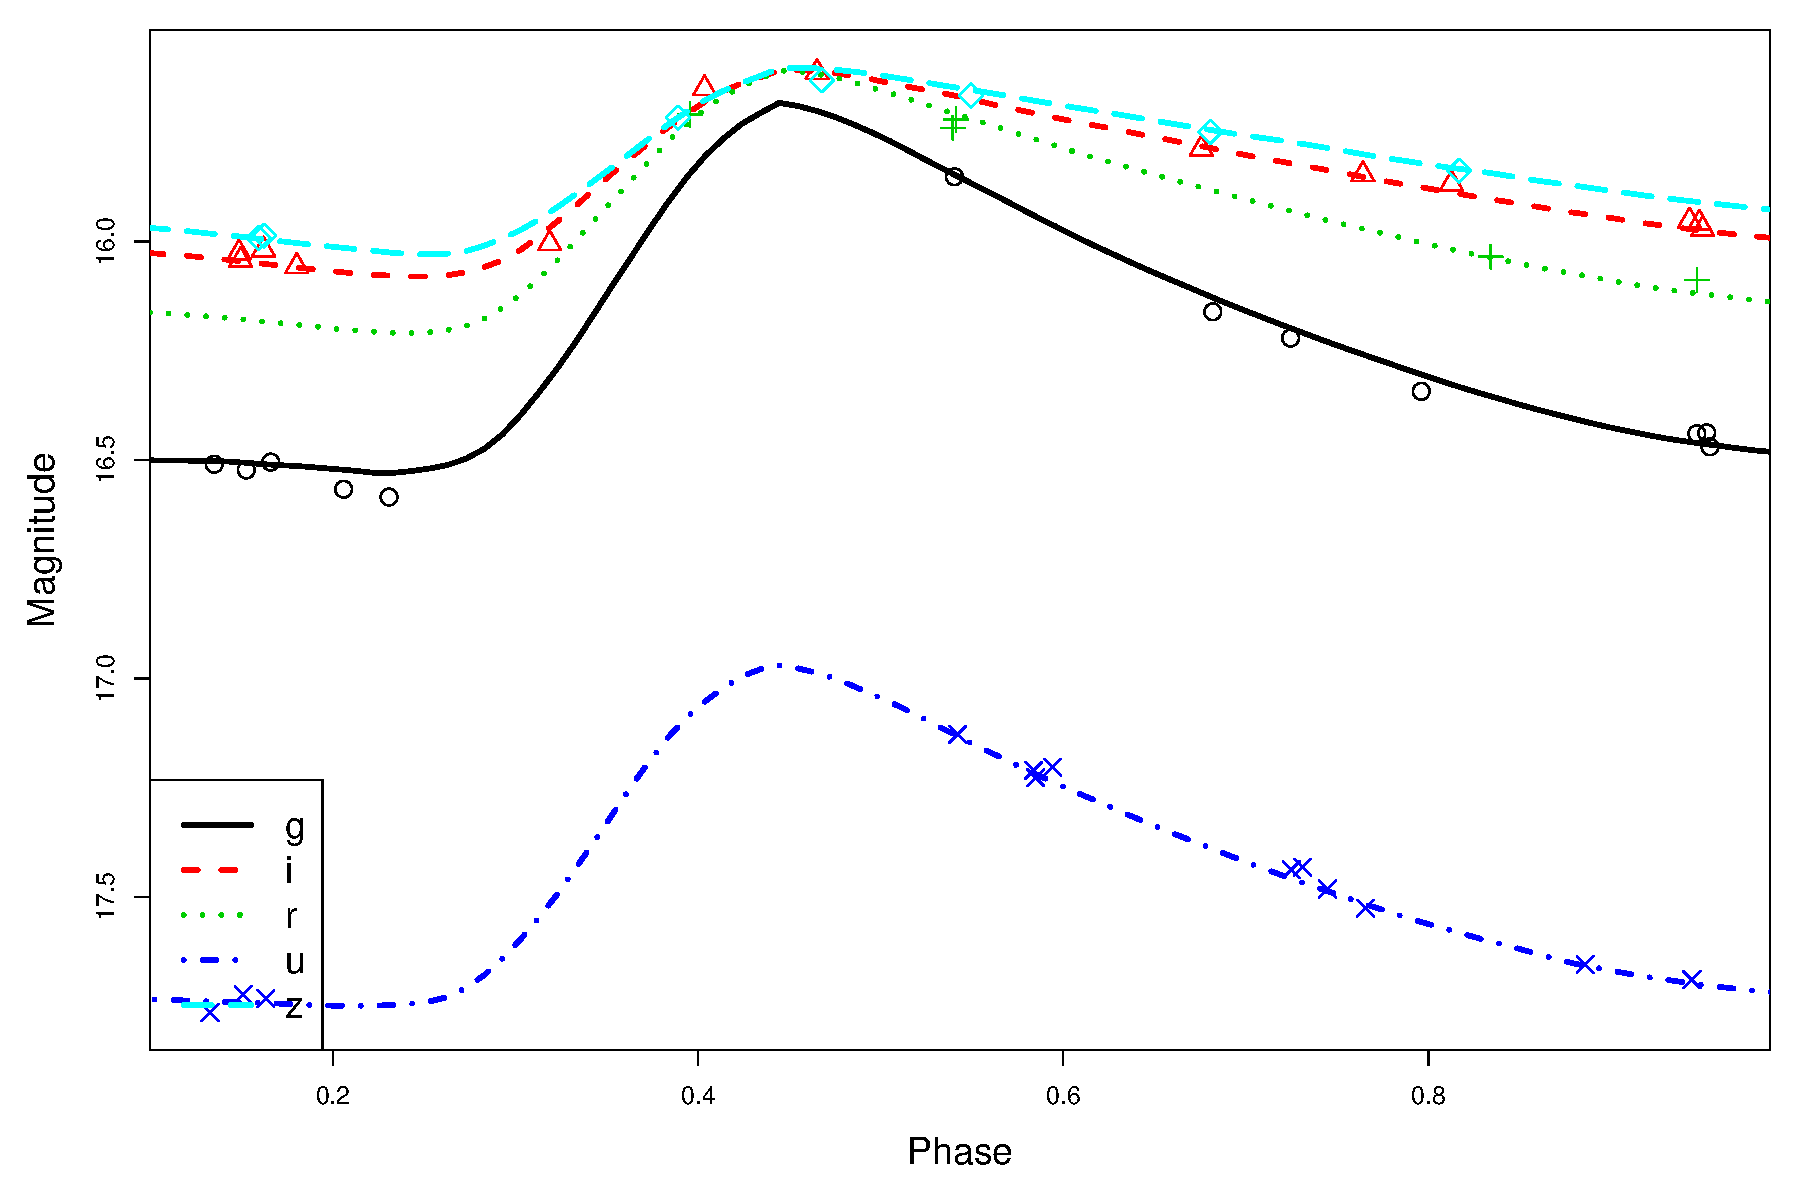
\includegraphics[width=0.7\linewidth]{2_one.pdf}
\captionof{figure}{Downsampled SDSS Strip 82 RR Lyrae with Model Fit \label{fig:sdss_down_fit}}
\end{center}\vspace{1cm}



\end{itemize}

\section*{Ongoing and Future Work}

\begin{itemize}
\item Current algorithm for maximizing likelihood only returns parameter estimates. Future implementation will quantify uncertainty in parameter estimates.
\item Develop goodness--of--fit statistics so algorithm can report probability that light curve is in fact RR Lyrae.
\item The Dark Energy Survey is currently collecting data. Will apply model to $\sim$ 1 million DES variable stars.
\item Use result of DES RR Lyrae search to construct maps of Milky Way halo. Possible discovery of Milky Way satellite galaxies or other structures. Compare results with cosmological simulations.
\end{itemize}





 %----------------------------------------------------------------------------------------
%	REFERENCES
%----------------------------------------------------------------------------------------

\nocite{*} % Print all references regardless of whether they were cited in the poster or not
\bibliographystyle{plain} % Plain referencing style
\bibliography{sample} % Use the example bibliography file sample.bib


\end{multicols}
\end{document}
